\documentclass[margin=.2cm]{standalone}

\usepackage{tikz}
\usepackage{algorithm}
\usetikzlibrary{calc,arrows}

\begin{document}

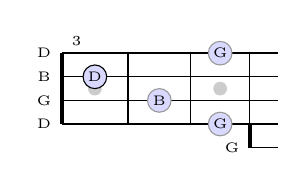
\begin{tikzpicture}[
    ynode/.style={draw=red!50,circle,fill=red!50,scale=.35,inner sep=1pt,minimum size=1.7em}]

  %%%% Draw the base and set coordinates %%%%
  \begin{scope}[xscale=-15,yscale=.3,line width=.5]

    \def\plushalf[#1]{\fpeval{0.5 + #1}}
    \def\fretname[#1]{\coordinate (fret#1) at (\fpeval{0.9875}, 5.5) }
    \def\nutoffset{0.015}
    \def\fifthnutx{0.840896415249188} 

    \xdef\x{1}

    \coordinate (Nut-5) at (\fpeval{1.0 + \nutoffset},                5);
    \coordinate (Nut-4) at (\fpeval{1.0 + \nutoffset},                4);
    \coordinate (Nut-3) at (\fpeval{1.0 + \nutoffset},                3);
    \coordinate (Nut-2) at (\fpeval{1.0 + \nutoffset},                2);
    \coordinate (Nut-1) at (\fpeval{\fifthnutx + \nutoffset},        1);

    \draw[line width=1.5] (1,2) -- (1,5);
\draw[line width=1.5] (\fifthnutx,1) -- (\fifthnutx,2); % fifth string peg
    \foreach \fret in {3,...,4}{

      %% define coordinate for fret label
      \fretname[\fret];
  
      %% Set coordinate for each string
      \foreach \str in {1,...,5}{
        \coordinate (\str-\fret) at (0.97193715634*\x,\str);
        \coordinate (plushalf\str-\fret) at (0.97193715634*\x,\plushalf[\str]);
      }
      %% Set coordinate for the text above
      \coordinate (Top-\fret) at (0.97193715634*\x,7);
      %% Compute the position of the fret
      \pgfmathsetmacro\x{\x * 0.94387431268}
      \xdef\x{\x}
      %% Draw the fret
      \draw[black] (\x,2) -- (\x,5);
    }
    \foreach \fret in {5,...,5}{
      %% Set coordinate for each string
      \foreach \str in {1,...,5}{
        \coordinate (\str-\fret) at (0.97193715634*\x,\str);
        \coordinate (plushalf\str-\fret) at (0.97193715634*\x,\plushalf[\str]);
      }
      %% Set coordinate for the text above
      \coordinate (Top-\fret) at (0.97193715634*\x,7);
      %% Compute the position of the fret
      \pgfmathsetmacro\x{\x * 0.94387431268}
      \xdef\x{\x}
      %% Draw the fret
      \draw (\x,2) -- (\x,5);
      \draw (\x,1) -- (\x,2);
    }
    %% Draw each string
    \foreach \str in {2,...,5}{
      \draw (1,\str) -- (0.97153194115*\x,\str);
      \coordinate (start\str) at (1,\str);
    }
    \foreach \str in {1,...,1}{
      \draw (\fifthnutx,\str) -- (0.97153194115*\x,\str);
      \coordinate (start\str) at (1,\str);
    }
  \end{scope}
  %% Draw the inlay circles
  \foreach \f in {3,5} {
    \draw[black!20,fill=black!20] ($(3-\f)!.5!(4-\f)$) circle (.08);
  }
  \foreach \f in {} {
    \draw[black!20,fill=black!20] (plushalf2-12) circle (.08) (plushalf4-12) circle (.08);
  }
  \draw[black!50, text=black] (fret3) node {\tiny 3 };
  %% label nut
  \draw[black!100] (Nut-5) node {\tiny D};
  \draw[black!100] (Nut-4) node {\tiny B};
  \draw[black!100] (Nut-3) node {\tiny G};
  \draw[black!100] (Nut-2) node {\tiny D};
  \draw[black!100] (Nut-1) node {\tiny G};
    % do a G major chord
  \draw[black!100,fill=blue!15]            (4-3) circle [radius=.15] node {\tiny D};
  \draw[black!40, text=black,fill=blue!15] (5-5) circle [radius=.15] node {\tiny G};
  \draw[black!40, text=black,fill=blue!15] (2-5) circle [radius=.15] node {\tiny G};
  \draw[black!40, text=black,fill=blue!15] (3-4) circle [radius=.15] node {\tiny B};

\end{tikzpicture}
\end{document}
